\documentclass{beamer}
\usetheme{Madrid}
\usepackage[italian]{babel}
\usepackage[latin1]{inputenc}
\usepackage[T1]{fontenc}
\usepackage{amsmath,amsfonts,amssymb,amsthm}
\usepackage{tikz-network}
\usepackage{graphics}
\usepackage{pgfplots}
 \pgfplotsset{compat=newest}
  \usetikzlibrary{plotmarks}
  \usetikzlibrary{arrows.meta}
  \usepgfplotslibrary{patchplots}
  \usepackage{grffile}
\usepackage{tikz}
\beamertemplatenavigationsymbolsempty
\pgfplotsset{plot coordinates/math parser=false}
  \newlength\figureheight
 \newlength\figurewidth

\newcommand{\spa}{\mathbin{\textcolor{white}{-}}} 
\newcommand{\angol}[1]{\langle #1 \rangle}
\newcommand{\tonde}[1]{\left( #1 \right)}
\theoremstyle{definition}
\newtheorem{defn}{Definizione}
\theoremstyle{plain}
\newtheorem{thm}{Teorema}
\usepackage{appendixnumberbeamer} 

\title[Discussione Tesi Triennale]{Il Modello Epidemiologico SIR \\ sulle Reti Complesse}
\author{Simmaco Di Lillo}
\date[24 settembre 2021]{Discussione Tesi Triennale in Matematica,\\
24 settembre 2021}
\institute{Universit\`a di Pisa}
\logo{
\includegraphics[width=15mm]{Figure/stemma_unipi.png}}

\begin{document}
\begin{frame}
\titlepage
\end{frame}

\begin{frame}
\frametitle{Il modello SIR scalare}
    Il modello SIR \`e un modello compartimentale: la popolazione viene suddivisa in $3$ classi 
    \begin{itemize}
    \item $S$: i suscettibili;
    \item $I$: gli infetti;
    \item $R$: i rimossi.
    \end{itemize}
\end{frame}

\begin{frame}{Il modello SIR scalare}
\begin{figure}
\centering
\begin{tikzpicture}
  \Vertex[x=0,shape = rectangle,label=S,size=1]{S}
  \Vertex[x=3,shape = rectangle,label=I,size=1]{I}
  \Vertex[x=6,shape = rectangle,label=R,size=1]{R}
  \Edge[Direct,label=$\tau  I$](S)(I)   \Edge[Direct,label = $\gamma$](I)(R)
  \end{tikzpicture}
  \caption{Schema del modello SIR.}
   \end{figure}
    
  \begin{columns}
  \begin{column}{0.5\textwidth}
  Assunzioni :
  \begin{itemize}
  \item $N$: numero di individui  (costante)  \item $\tau$: tasso di contatto 
  \item $\gamma$: tassi di recupero
  \end{itemize}
  \end{column}
  \pause
  \begin{column}{0.5\textwidth}
  \begin{equation*}
  \begin{aligned}
      \dot{S} =& -\tau S I \\
      \dot{I} = & \spa \tau S I - \gamma I  \\
      \dot{R} = & \spa \gamma I 
      \end{aligned}
  \end{equation*}
  \end{column}
  \end{columns}
 
\end{frame}
\begin{frame}
\frametitle{Il modello SIR bottom-up su una rete}
\framesubtitle{Un primo esempio}
\pause
Notazione:
\begin{itemize}
\item $\angol{A_i}(t)$: probabilit\`a che il nodo $i$ si trovi nello stato $A$ al tempo $t$ 
\item $\angol{A_iB_j}(t)$: probabilit\`a che il nodo $i$ si trovi nello stato $A$ e il nodo $j$ in $B $ al tempo $t$ 
\end{itemize}
\pause
\begin{figure}
\centering
\begin{tikzpicture}
  \Vertex[x=0,label=$1$,size=1]{S}
  \Vertex[x=3,label=$2$,size=1]{I}
  \Vertex[x=6,label=$3$,size=1]{R}
  \Edge(S)(I)   \Edge(I)(R)
  \end{tikzpicture}
  \end{figure}
  Come si infettano?
  \begin{itemize}
      \item<3-> Il nodo $1$ ha una sola fonte d'infezione.\\
      \only<3>{$\langle S_1\rangle $ diminuisce con un tasso di $\tau \angol{S_1 I_2}$}
      \item<4-> Il nodo $2$ ne ha due.\\
       \only<4>{$\langle S_2\rangle $ diminuisce con un tasso di $\tau \angol{I_1 S_2} +\tau \angol{S_2 I_3}$}
      \item<5-> Anche il  nodo $3$ ne ha una sola.\\
      \only<5>{$\langle S_3\rangle $ diminuisce con un tasso di $\tau \angol{I_2 S_3} $}
  \end{itemize}
\end{frame}
\begin{frame}
    \frametitle{Il modello SIR bottom-up su una rete}
\framesubtitle{Un primo esempio}
\begin{equation*}
\begin{aligned}
	\dot{\angol {S_1}} = & -\tau \angol{ S_1 I_2}, 
\quad &
	\dot{\angol {I_1}} = & \tau \angol{S_1 I_2}-\gamma \angol{I_1}, 
\\
	\dot{\angol {S_2}} = & -\tau \tonde{ \angol{ I_1 S_2} + \angol{S_2I_3}},	
\quad & 
	\dot{\angol {I_2}} = & \tau \tonde{ \angol{ I_1 S_2} + \angol{S_2I_3}}-\gamma \angol{I_2},
\\
	\dot{\angol {S_3}} = & -\tau \angol{ I_2 S_3},
\quad & 
	\dot{\angol {I_3}} = & \tau \angol{ I_2 S_3}-\gamma \angol{I_3},
\end{aligned}
\end{equation*}
\pause
Tale sistema \alert{non \`e chiuso}. Dipende da alcune coppie. 
\end{frame}
\begin{frame}
\frametitle{Il modello SIR bottom-up su una rete}
\framesubtitle{Un primo esempio}
Come evolvono nel tempo le coppie?
    \begin{equation*}
\begin{aligned}
	\dot{\angol{S_1I_2}}=&\spa\tau\angol{S_1S_2I_3} - \tonde{ \tau + \gamma}\angol{S_1 I_2},
\\
	\dot{\angol{I_1S_2}}=&-\tau\angol{I_1S_2I_3} - \tonde{ \tau + \gamma}\angol{I_1 S_2},
\\
	\dot{\angol{S_2I_3}}=&-\tau\angol{I_1S_2I_3} - \tonde{ \tau + \gamma}\angol{S_2 I_3},
\\
	\dot{\angol{I_2S_3}}=&\spa\tau\angol{I_1S_2S_3} - \tonde{ \tau + \gamma}\angol{I_2 S_3}.
	\end{aligned}
\end{equation*}
\pause
e le triple?
\begin{equation*}
    \begin{aligned}
        	\dot{\angol{S_1S_2I_3}}=&-\tonde{\tau + \gamma}\angol{S_1S_2I_3},
\\
	\dot{\angol{I_1S_2I_3}}=&-\tonde{2\tau + 2\gamma}\angol{I_1S_2I_3},
\\
	\dot{\angol{I_1S_2S_3}}=&-\tonde{\tau + \gamma}\angol{I_1S_2S_3}.
 \end{aligned}
\end{equation*}
\end{frame}
\begin{frame}
      \frametitle{Il modello SIR bottom-up su una rete}
\framesubtitle{Modello generale}
Sia $G = \left( g_{ij}\right)$ la \alert{ matrice di adiacenza} del grafo $G$. L'epidemia si diffonde sul grafo nel seguente modo 
\begin{equation*}
\begin{aligned}
	 \dot{\angol{ S_i}}=& - \tau \sum_{j=1\atop{j\neq i }}^N g_{ij} \angol{ S_i I_j},\\
	 \dot{\angol{I_i}} =&\spa \tau \sum_{j=1\atop{j\neq i}}^N  g_{ij} \angol{ S_i I_j} -\gamma_i \angol{I_i},
\end{aligned}
\end{equation*}
\end{frame}
\begin{frame}
\frametitle{Il modello SIR bottom-up su una rete}
\framesubtitle{Chiusura alle coppie}
\begin{defn}[Coefficienti di correlazione]
Siano $A,B \in \{ S, I, R\}$ e $(i,j)\in E $ allora 
$$ C_{A_i B_j} = \frac{ \angol{ A_i B_j}}{\angol{A_i} \angol{B_j}} $$ 
\end{defn}
\pause
Nel modello SIR 
\begin{itemize}
\item $C_{I_i I_j} \geq 1 $ 
\item $C_{S_iI_j}\leq 1 $ 
\end{itemize}
\pause
Per ottenere un modello chiuso ma \alert{non esatto} assumeremo l'indipendenza a livello delle coppie ovvero:
$$ \angol{ A_i B_j } \approx \angol{ A_i }\angol{B_j} \quad \forall A, \, B \in \{ S, \, I,\, R\} \text{ e } \forall (i,j) \in E $$

\end{frame}
\begin{frame}
\frametitle{Il modello SIR bottom-up su una rete}
\framesubtitle{Chiusura alle coppie}
\begin{columns}
\begin{column}{0.5\textwidth}
\begin{figure}
    \centering
    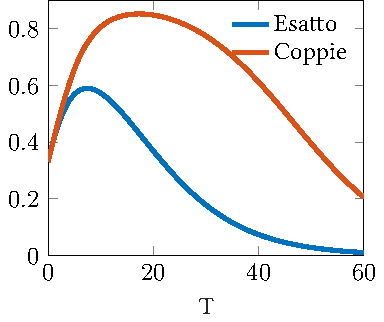
\includegraphics[scale=0.8]{Figure/Coppie_Prevalenza}
    \caption{Prevalenza nei  due modelli. }
\end{figure}
    \end{column}
    \begin{column}{0.5\textwidth}
    Riportiamo la definizione data dall'OMS nel 1959:
    \begin{quote}La \textit{prevalenza} indica il numero di individui malati in una determinata popolazione, senza nessuna distinzione tra nuovi e vecchi casi. La \alert{prevalenza puntiforme}  \`e solitamente espressa come una frazione: il denominatore \`e il numero della
    popolazione.	
    \end{quote}
    \end{column}
\end{columns}
\end{frame}
{
\logo{}
\begin{frame}
\frametitle{Il modello SIR bottom-up su una rete}
\framesubtitle{Approccio generale alla chiusura}
Diamo due importanti definizioni
    \begin{defn}[cut-vertex]
    Sia $G=(V,E)$ un grafo connesso. $v\in V$ \`e un \textit{cut-vertex} se il grafo senza il nodo $v$ risulta sconnesso.
    \end{defn}
    \pause 
    \begin{defn}[Probabilit\`a condizionale]
    Siano $A,B$ due eventi di uno spazio di probabilit\`a con $\mathbb{P}(B)>0$. Si dice \textit{probabilit\`a condizionale} di $A$ dato $B$ la quantit\`a
    $$ \mathbb{P}(A\, \vert B) = \frac{ \mathbb{P}(A\cap B)}{\mathbb{P}(B)}.$$
    \end{defn}
\end{frame}

\begin{frame}
\frametitle{Il modello SIR bottom-up su una rete}
\framesubtitle{Approccio generale alla chiusura}
\begin{thm}[\small{Kiss, Morris, Se\'elley, Simon, Wilkinson, J.~Math.~Biol.~2015}]
Sia $G=(V,E)$ un grafo e $F=\{ v_1, \dots, v_k\}$ un sottoinsieme connesso di vertici e sia $v_i$ un suo cut-vertex. Poniamo  $$ F_1 = \{ v_1, \dots, v_{i-1}\} \text{ e }  F_2 =\{ v_{i+1}, \dots, v_k\}.$$ 
Se ogni cammino che connette un nodo in $F_1$ ad uno in $F_2$ passa da $v_i$ allora: 
\begin{equation*}angol{ Z_{v_1}\dots Z_{v_{i-1}} S_{v_i} Z_{v_{i+1}} \dots Z_{v_k}} = \angol{ Z_{v_1}\dots Z_{v_{i-1}} S_{v_i}} \angol{S_{v_i}  Z_{v_{i+1}} \dots Z_{v_k}}	
\end{equation*}
dove $Z\in \{ S,I,R\}$. 
\end{thm}
\end{frame}

\begin{frame}
\frametitle{Il modello SIR bottom-up su una rete}
\framesubtitle{Approccio generale alla chiusura}

\small {
\begin{thm} $[...]$
\begin{equation*}\angol{ Z_{v_1}\dots Z_{v_{i-1}} S_{v_i} Z_{v_{i+1}} \dots Z_{v_k}} = \angol{ Z_{v_1}\dots Z_{v_{i-1}} S_{v_i}} \angol{S_{v_i}  Z_{v_{i+1}} \dots Z_{v_k}}	
\end{equation*}
\end{thm}}


\begin{proof}
\only<1>{Se $\angol{S_{v_i}}=0$ allora l'uguaglianza risulta banalmente vera.\\ }
\pause Sia $\angol{S_{v_i}}\neq 0 $
\pause
$$ \angol{ Z_{v_1}\dots Z_{v_{i-1}} S_{v_i} Z_{v_{i+1}}\dots Z_{v_k}} = \angol{ Z_{v_1}\dots Z_{v_{i-1}} S_{v_i} Z_{v_{i+1}}\dots Z_{v_k}\, \vert \, S_{v_i}} \angol{S_{v_i}}.$$
\pause
Notiamo che 
$$ \angol{ Z_{v_1}\dots Z_{v_{i-1}} S_{v_i} Z_{v_{i+1}}\dots Z_{v_k}\, \vert \, S_{v_i}} =$$
$$=\angol{ Z_{v_1}\dots Z_{v_{i-1}} S_{v_i} \, \vert\, S_{v_i}} \angol{S_{v_i}Z_{v_{i+1}}\dots Z_{v_k}\, \vert \, S_{v_i}}.$$ 
Ogni percorso da $F_1$ a $F_2$ deve passare attraverso $v_i$. Poich\`e $v_i$ \`e suscettibile  la trasmissione non pu\`o avvenire tra un nodo in $F_1$ ed uno in $F_2$.\\\pause
Riapplicando la definizione di probabilit\`a condizionale la tesi 
\end{proof}

\end{frame}
}
\begin{frame}
\frametitle{Il modello SIR bottom-up su una rete}
\framesubtitle{Approccio generale alla chiusura}
\begin{itemize}
	\item<1->\alt<1>{Con una \alert{visita in profondit\`a} si trovano tutti i cut-vertex di $G$.}{Con una visita in profondit\`a si trovano tutti i cut-vertex di $G$.}
	\item<2->\alt<2>{Si divide la rete originale in \alert{sottoreti} connesse a due a due scollegate. Le sottoreti vengono create in modo che i cut-vertex siano mantenuti in tutte le sottoreti generate.}{Si divide la rete originale in sottoreti ...}
	\item<3-> \alt<3>{Per ogni nodo $i$ delle sottoreti, si ha}{ Per ogni nodo $i$ delle sottoreti ...}
	\only<3>{
	\begin{equation*}
	\begin{aligned}
\dot{\angol{S_i}} &= -\tau \sum_j g_{ij} \angol{S_iI_j},\\
\dot{\angol{I_i}} &= \tau \sum_j g_{ij} \angol{S_iI_j}-\gamma\angol{I_i},\\
\dot{\angol{R_i}} &= 1 -\angol{S_i} -\angol{I_i}.
		\end{aligned}
	\end{equation*}
	Si possono trovare  equazioni simili anche per le strutture di ordine maggiore (coppie, triple, ...)}
	\item<4-> Nella gerarchia che si verr\`a a creare, se appare un termine composto da  vertici di sottoreti diverse allora in esso \`e presente un cut-vertex suscettibile. Usando il Teorema precedente  \`e possibile esprimere questo termine usando \alert{termini pi\`u semplici}.
\end{itemize}

\end{frame}
\begin{frame}
\frametitle{Il modello SIR bottom-up su una rete}
\framesubtitle{La rete lollipop}
\begin{columns}
\begin{column}{0.5\textwidth}
   \begin{figure}
\centering
\begin{tikzpicture}[scale=0.8]
\Vertex[label=1]{1}
\Vertex[label=2,y=-2]{2}
\Vertex[label=3, y=-1, x=1.73]{3}
\Vertex[label=4, y=-1, x= 3.73]{4}
\Edge(1)(2) \Edge(2)(3) \Edge(1)(3) \Edge(3)(4)
\end{tikzpicture}
\caption{Rete lollipop.}
\end{figure}

\end{column}
\pause
\begin{column}{0.5\textwidth}  %%<--- here
\begin{figure}[!htb]
\centering
\begin{tikzpicture}[scale=0.8]
\Vertex[label=1]{1}
\Vertex[label=2,y=-2]{2}
\Vertex[label=3, y=-1, x=1.73,color=gray,opacity=0.3]{3}
\Vertex[label=3, y=-1, x= 3.73,color=gray,opacity=0.3]{33}
\Vertex[label=4, y=-1, x=5.73]{4}
\Edge(1)(2) \Edge(2)(3) \Edge(1)(3) \Edge(33)(4)
\end{tikzpicture}
\caption{Rete lollipop: decomposizione.}
\end{figure}
\end{column}
\end{columns}
\pause
\begin{equation*}
 \begin{aligned}	
 \dot{\angol{S_1I_3}}&=
 \pause  \tau \tonde{ \angol{S_1I_2S_3} +
  \alt<8>
  {\alert{\angol{S_1S_3I_4}}}
  {\angol{S_1S_3I_4}} }
   \pause -  \tau  \angol{S_1I_3} \pause - \gamma\angol{S_1 I_3}\pause -\tau \angol{ S_1 I_2 I_3}= \\ \pause
 &= \tau \tonde{ \angol{S_1I_2S_3} +
 \alt<8>{\alert{
  \frac{\angol{S_1S_3}\angol{S_3 I_4}}{\angol{S_3}}}}
  {\frac{\angol{S_1S_3}\angol{S_3 I_4}}{\angol{S_3}}  }
  } -\tonde{ \tau + \gamma} \angol{S_1I_3} - \tau \angol{S_1I_2S_3}
 \end{aligned}
 \end{equation*}
\pause
Grazie al Teorema,  il numero di equazioni passa da $35$ a $27$
\end{frame}
\begin{frame}
\frametitle{Errori usando le chiusure}

\begin{columns}
\begin{column}{0.5\textwidth} 
 \begin{figure}
\centering
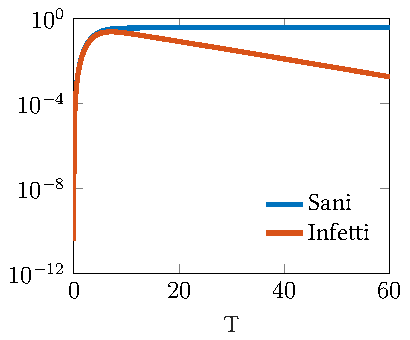
\includegraphics[width=0.85\textwidth]{Figure/figure10}
\caption{Chiusura alle coppie.}
\end{figure}
\end{column}
\begin{column}{0.5\textwidth}
\pause
 \begin{figure}
\centering
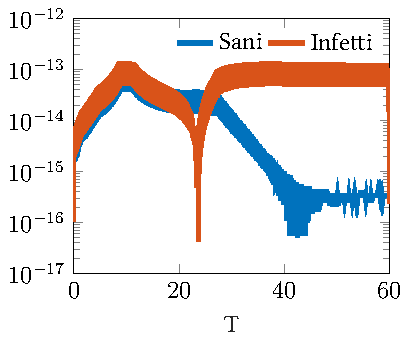
\includegraphics[width=0.85\textwidth]{Figure/figure9}
\caption{Chiusura con cut-vertex.}
\end{figure}
\end{column}
\end{columns}
\end{frame}
\begin{frame}
\frametitle{La rete stradale del Minnesota}
\begin{columns}
\begin{column}{0.5\textwidth}
\begin{figure}
\centering
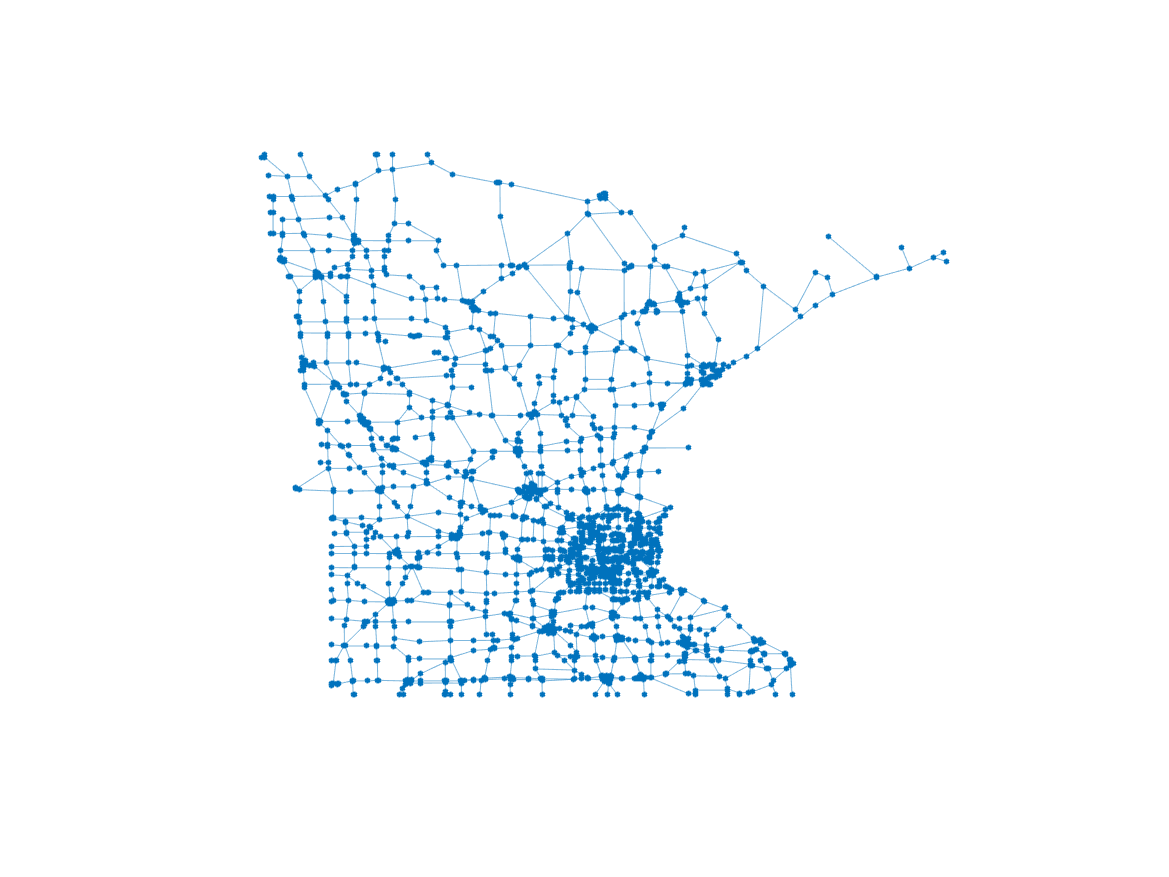
\includegraphics[width=0.85\textwidth]{Figure/minnesota}
\caption{La rete stradale del Minnesota.}
\end{figure}
\end{column}
\begin{column}{0.5\textwidth}
Abbiamo integrato il modello chiuso alle coppie 
\begin{itemize}
\item funzione \texttt{ode15s} di MATLAB
\item Tolleranza assoluta: $1e-12$
\item Tolleranza relativa: $1e-12$
\item Intervallo temporale: $[0, 160]$
\item Tasso d'infezione: $\tau = 0.3$
\item Tasso di rimozione: $\gamma = 0.1$
\end{itemize}
Le condizioni iniziali sono stati puri: un nodo certamente infetto gli altri certamente sani 
\end{column}
\end{columns}
\end{frame}
\begin{frame}
\frametitle{La rete stradale del Minnesota}
\framesubtitle{Sperimentazione numerica}
\begin{columns}
\begin{column}{0.5\textwidth} 
 \begin{figure}
\centering
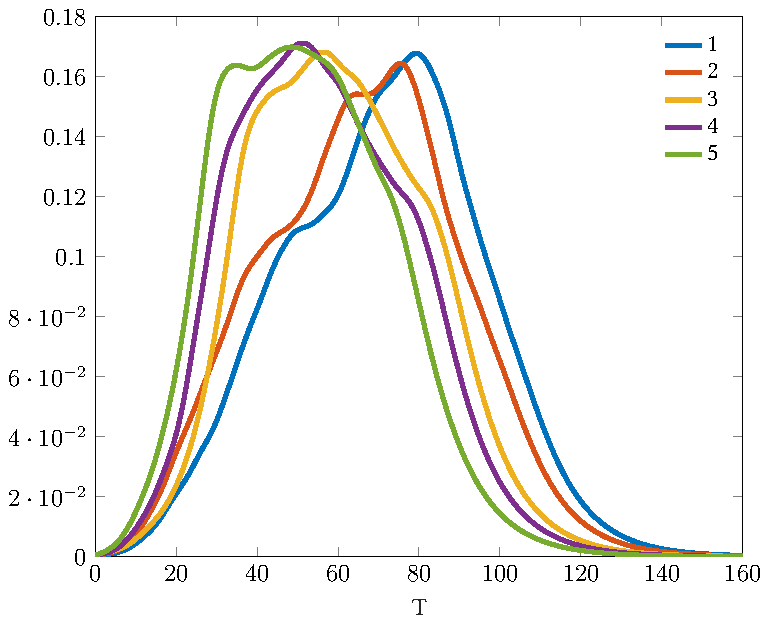
\includegraphics[width=0.85\textwidth]{Figure/minnesota_prevalenza}
\caption{Prevalenza e grado.}
\end{figure}
\end{column}
\begin{column}{0.5\textwidth}
\pause
 \begin{figure}
\centering
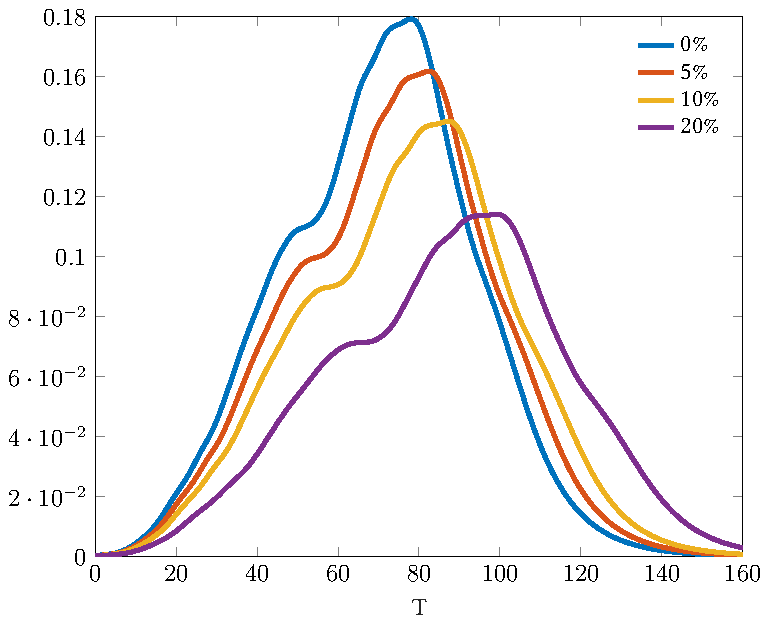
\includegraphics[width=0.85\textwidth]{Figure/minnesota_immunizzazione}
\caption{Immunizzazione.}
\end{figure}
\end{column}
\end{columns}
\end{frame}

\begin{frame}
\begin{center}
\begin{huge}
Grazie per l'attenzione.\\
Tutto il materiale \`e reperibile sul repository:\\
\url{https://github.com/simmaco99/Tesi}
\end{huge}
\end{center}
\end{frame}



\end{document}
